\section{IIO Subsystem}

\begin{frame}
   {Overview}

   \begin{itemize}
      \item
	      The Linux IIO subsystem is a framework to support sensors and any type of device with ADCs or DACs
      \item
	      \url{https://www.kernel.org/doc/html/v5.0/driver-api/iio/intro.html}
      \item
	      IIO provides a core framework to support device drivers in a common manner
	\item
		IIO also provides an interface for in-kernel users of IIO devices
	\item
		IIO provides a high-latency userspace interface via sysfs
	\item
		IIO provides an efficient buffered interface via character device
   \end{itemize}
\end{frame}

\begin{frame}
	{IIO architecture}
	     \begin{figure}[H]
		     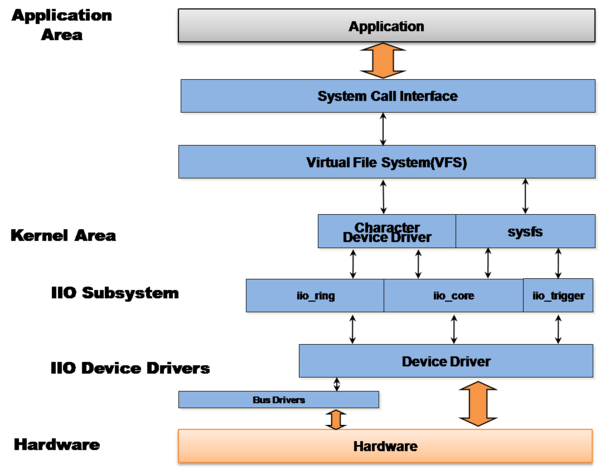
\includegraphics[width=4in]{IMAGES/iio_block_view}
				       \caption{IIO architecture}
	     \end{figure}
\end{frame}

\begin{frame}
	{IIO concepts}
   \begin{itemize}
	   	\item Producer/Consumer model
		   \begin{itemize}
			   \item Sensor/ADC drivers are producers of samples.
			   \item In-kernel drivers or userspace clients are consumers of samples.
		   \end{itemize}
		\item Ring buffer (efficient buffered access to samples)
		   \begin{itemize}
			   \item Hardware and software circular buffer support for producers to place samples.
		   \end{itemize}
      		\item Triggers (external events to \textbf{trigger} capture of a sample)
		   \begin{itemize}
			   \item GPIO
			   \item RTC
			   \item sysfs file
		   \end{itemize}
      		\item Scaled samples
		   \begin{itemize}
			   \item Ability to provide both raw samples and scaled (in units relevant to the sensor e.g. mA, mV, lumens, foot pounds per fortnight, etc.)
    		   \end{itemize}
   \end{itemize}
\end{frame}

\begin{frame}
	{IIO userspace ABI}

	The canonical ABI documentation is here \url{https://git.kernel.org/pub/scm/linux/kernel/git/torvalds/linux.git/tree/Documentation/ABI/testing/sysfs-bus-iio}

	Focusing on the polled sysfs interface:
	\begin{itemize}
		\item IIO device nodes
			\begin{itemize}
				\item /sys/bus/iio/devices/iio:deviceN
			\end{itemize}
		\item IIO device attribute nodes
			\begin{itemize}
				\item /sys/bus/iio/devices/iio:deviceN/in\_*\_raw
				\item /sys/bus/iio/devices/iio:deviceN/in\_*\_scale
				\begin{itemize}
					\item Variations for each type of sample (voltage, current, power, temperature
				\end{itemize}
			\end{itemize}
	\end{itemize}
\end{frame}

\begin{frame}
    {IIO temp sensor example}

	Example graciously provided by Matt Ranostay from his \url{https://elinux.org/images/b/ba/ELC_2017_-_Industrial_IO_and_You-_Nonsense_Hacks!.pdf} presentation.

	\begin{rawscriptsize}
$ cd /sys/bus/iio/devices/iio:device0
$ cat in_temp_raw
98
$ cat in_temp_ambient_raw
416
$ cat in_temp_scale
250
$ cat in_temp_ambient_scale
62.500000
	\end{rawscriptsize}
\end{frame}

\begin{frame}
    {libiio}

	\textbf{libiio} is a higher level userspace library for working with IIO devices. The official documentation is at \url{http://analogdevicesinc.github.io/libiio/}. It was created in response to the difficulty of working with the low-level IIO userspace ABI for buffered I/O management.

	\textbf{libiio} provides high level APIs to manage
	\begin{itemize}
		\item polled sysfs read/write attributes
		\item trigger events
		\item buffered samples
	\end{itemize}

	\textbf{libiio} is also used by the \textbf{iiod} server to provide networked access to IIO data and provides several utilities like \textbf{iio\_info} and \textbf{iio\_attr} for retrieving data from IIO.
\end{frame}
